{
\newcommand{\tr}{{\sf T}}
MATLABを用いて電力システムの時間応答をシミュレーションするプログラムを実装する方法について説明する。
電力系統の時間応答のシミュレーションは,機器の動特性を表す微分方程式と,
電力潮流の代数方程式を連立した微分代数方程式を解くことによって行われる。
そこで,まずは簡単な微分代数方程式を例に,その解き方を見てみよう。

\begin{例}[簡単な例題]\label{ex:dae_ex1}
\begin{figure}[t]
  \centering
  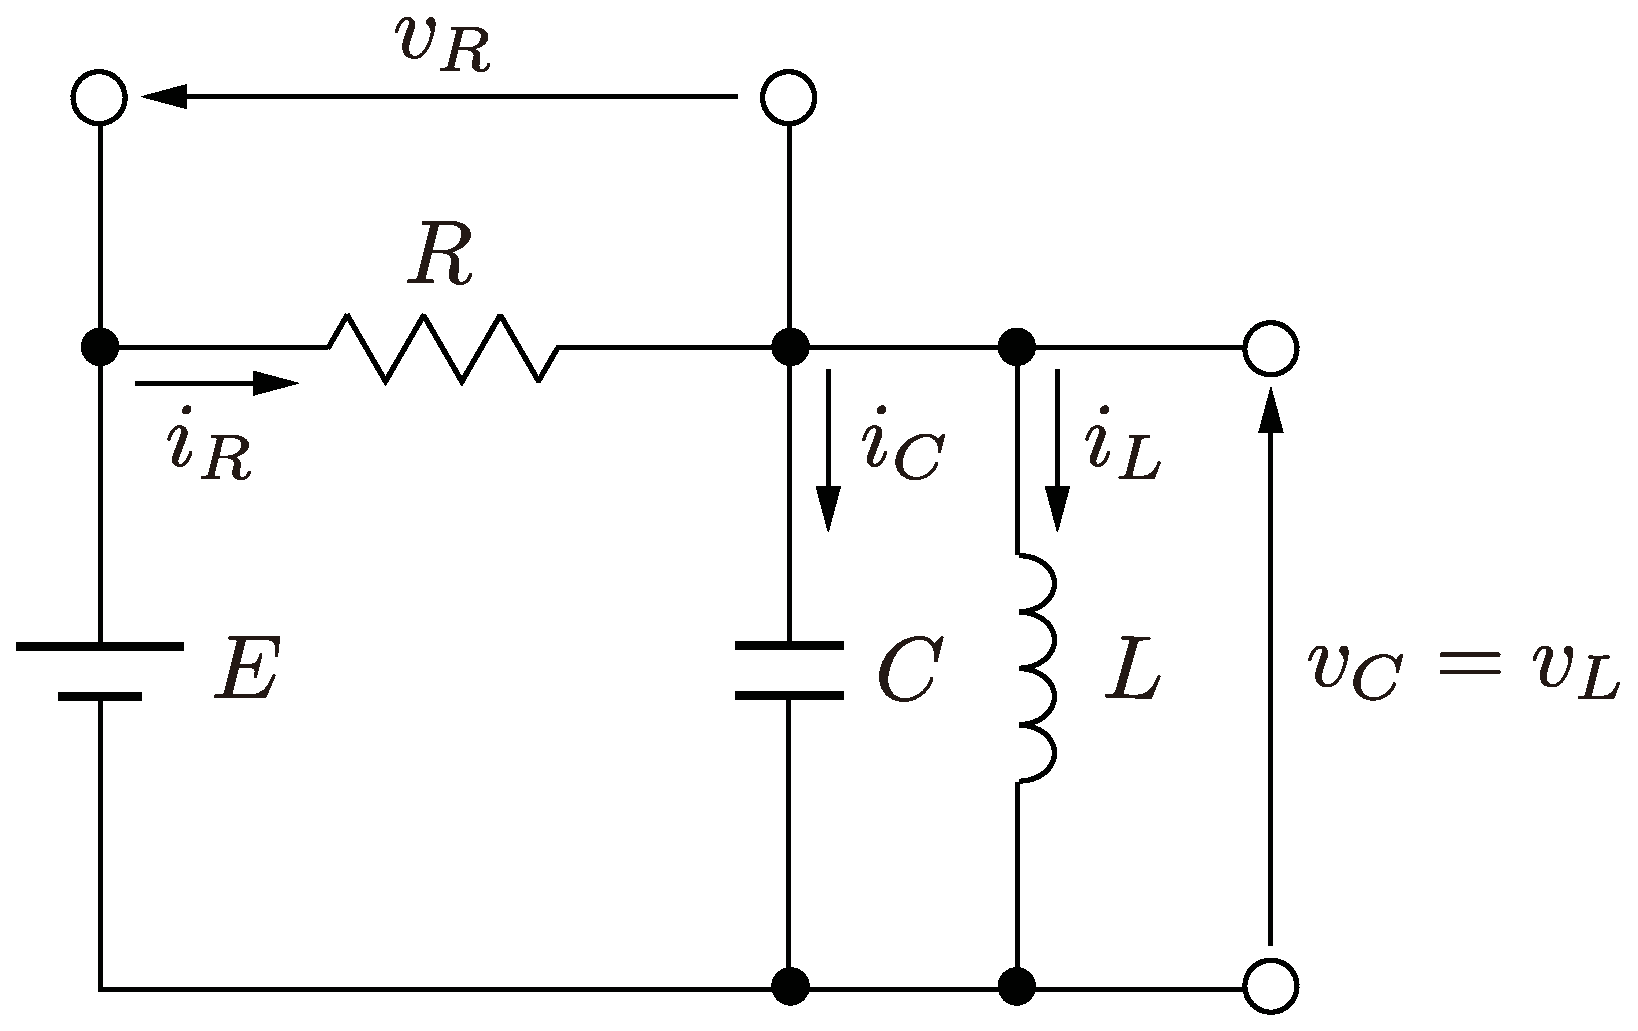
\includegraphics[width = .4\linewidth]{figs/circkawaguchi.eps}
  \medskip
  \caption{\textbf{微分代数方程式の例題:LC並列回路}}
  \label{fig:RLC}
  \medskip
\end{figure}
図\ref{fig:RLC}の簡単な電気回路において,$R=L=C=E=1$のときのシミュレーションを行うことを考える。
この回路の動的な要素はコイル$L$とコンデンサ$C$であり,その微分方程式は,
\begin{subequations}\label{eq:ex_de}
  \begin{align}
    L\dot i_L & = v_L \\
    C\dot v_C & = i_C
  \end{align}
\end{subequations}
である。ただし,初期値は$i_L(0)=0$,$v_C(0)=0$とする。
また,オームの法則とキルヒホッフの法則から,
\begin{subequations}\label{eq:ex_ae}
  \begin{align}
    v_R & =R i_R      \\
    i_R & = i_L + i_C \\
    v_L & = v_C       \\
    E   & = v_C + v_R
  \end{align}
\end{subequations}
という代数方程式が成り立つ。

このシステムは微分方程式と代数方程式が連立された
微分代数方程式である。
式\ref{eq:ex_ae}の代数方程式を用いて文字を消去すると,
等価な常微分方程式を得ることができる。
これはクロン縮約に対応し,得られる常微分方程式は,
\begin{subequations}\label{eq:ex1_ode}
  \begin{align}
    \dot{i}_L & = \frac{1}{L}v_C                     \\
    \dot{v}_C & = \frac{1}{RC}(E-v_C)-\frac{1}{C}i_L
  \end{align}
\end{subequations}
となる。まずは,この常微分方程式を解くプログラムを書いてみよう。
常備分方程式に対するMATLABのソルバとしては\verb|ode45|を用いるのが
一般的である。\verb|ode45|では,常微分方程式$\dot{x} = f(t, x)$
の関数$f(t, x)$を実装することにより常微分方程式を解くことができる。
式(\ref{eq:ex1_ode})の右辺を実装すると,プログラム\ref{program:ex1_ode}のようになる。
\begin{PROGRAMA}[count,title={func\_RLC\_ode.m}]\label{program:ex1_ode}
  \begin{verbatim}
function dx = func_RLC_ode(x, R, C, L, E)
vC = x(2);

diL = vC/L;
dvC = (E-vC)/R/C - iL/C;

dx = [diL; dvC];

end
\end{verbatim}
\end{PROGRAMA}
また,これを用いて\verb|ode45|を実行し,常微分方程式を解くプログラムは
プログラム\ref{program:main_ode1}となる。
\begin{PROGRAMA}[count,title={main\_RLC\_ode.m}]\label{program:main_ode1}
  \begin{verbatim}
R = 1;
L = 1;
C = 1;
E = 1;

func = @(t, x) func_rlc_ode(x, R, C, L, E);
x0 = [1; 1];
tspan = [0 30];

[t, x] = ode45(func, tspan, x0);
\end{verbatim}
\end{PROGRAMA}
このプログラムにおいて,出力された変数\verb|x|は,$i_L$と$v_C$の時系列を
並べたベクトルである。したがって,$i_C$や$i_R$などの他の変数については
式(\ref{eq:ex_ae})の代数方程式を用いて改めて計算する必要があることに注意しよう。

つぎに,クロン縮約を行わず,微分代数方程式を直接解くことを考える。
これには,物理的な代数方程式をそのまま用いることとができ,
複雑なシステムになっても記述が簡単である利点がある。
MATLABで微分代数方程式を解くことができるコマンドのひとつに\verb|ode15s|がある。
\verb|ode15s|は
\[
  M\dot{x} = f(x)
\]
という形で記述された微分代数方程式を対象とする。式\ref{eq:ex_de},\ref{eq:ex_ae}をこの形にあてはめると,
\[
  \begin{bmatrix}
    0 & L & 0 & 0 & 0 & 0 \\
    0 & 0 & 0 & 0 & 0 & C \\
    0 & 0 & 0 & 0 & 0 & 0 \\
    0 & 0 & 0 & 0 & 0 & 0 \\
    0 & 0 & 0 & 0 & 0 & 0 \\
    0 & 0 & 0 & 0 & 0 & 0 \\
  \end{bmatrix}
  \begin{bmatrix}
    \dot i_R \\\dot i_L\\\dot i_C\\\dot v_R\\\dot v_L\\\dot v_C
  \end{bmatrix}
  =\begin{bmatrix}
    v_L \\i_C\\v_R-R i_R\\i_R-i_L-i_C\\v_L-v_C\\E-v_C-v_R
  \end{bmatrix}
\]
となる。ここで,右辺の3番目以降の要素の順番は任意であることに注意しよう。
この右辺を実装するとプログラム\ref{program:DAE1}となる。

\begin{PROGRAMA}[count,title={func\_RLC\_DAE.m}]\label{program:DAE1}
  \begin{verbatim}
function dx = func_rlc_dae(x, R, C, L, E)

vR = x(1);
vL = x(2);
vC = x(3);
iR = x(4);
iL = x(5);
iC = x(6);

dvC = iC;
diL = vL;

con1 = vC-vL;
con2 = E-vC-vR;
con3 = iR-(iC+iL);
con4 = vR-iR*R;

dx = [dvC; diL; con1; con2; con3; con4];
end
\end{verbatim}
\end{PROGRAMA}
この関数を用いると,プログラム\ref{program:DAE1}のように微分代数方程式を解くことができる。
\begin{PROGRAMA}[count,title={main\_RLC\_DAE.m}]\label{program:DAE1}
  \begin{verbatim}
R = 1;
C = 1;
L = 1;
E = 1;

M = zeros(6, 6);
M(1, 2) = L;
M(2, 6) = C;

x0 = zeros(6, 1);
tspan = [0 30];

options = odeset('Mass', M);
func = @(t, x) func_RLC_DAE(x, R, C, L, E);
[t, y] = ode15s(func, tspan, x0, options); 
\end{verbatim}
\end{PROGRAMA}
このプログラムにおいて,10行目で初期状態をすべて0ととっているが,
意味を持つのは動的な要素の値のみ,すなわち,2番目と6番目の要素のみであり,
他の値については代数方程式を満たす値が\verb|ode15s|によって探索される。
また,解\verb|x|は,$v_R, v_L, v_C, i_R, i_L, i_C$の時系列を並べた行列であり,
常微分方程式に変換した場合と異なり,すべての物理量を含んでいる。

常微分方程式として解いた場合と微分代数方程式として解いた場合の$i_L$と$v_C$を図\ref{fig:solution_dae}
に示す。それぞれの図には\verb|ode45|と\verb|ode15s|の解の2本の線が表示してあるが,当然ながらこれらは完全に重なっている。
\begin{figure}[t]
  \centering
  {
    \begin{minipage}{0.49\linewidth}
      \centering
      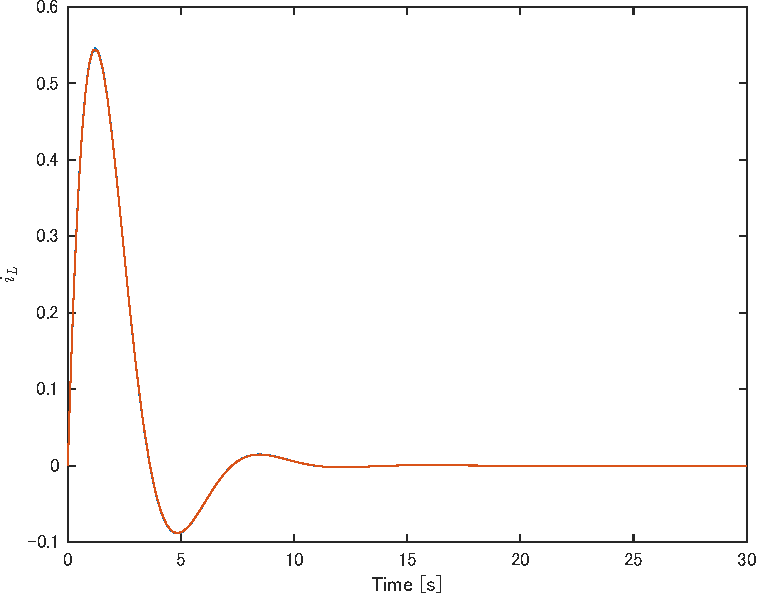
\includegraphics[width = 1.0\linewidth]{figs/i_L}
      \subcaption{$i_L$の時間応答}
    \end{minipage}
    \begin{minipage}{0.49\linewidth}
      \centering
      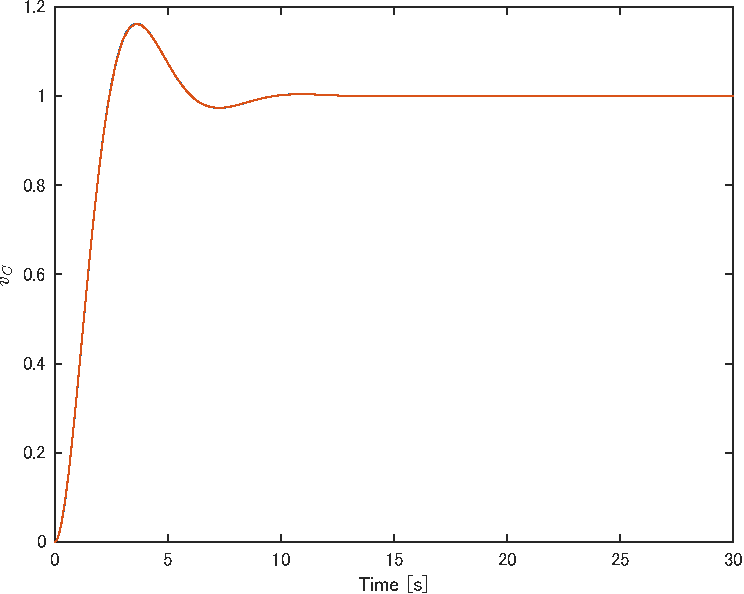
\includegraphics[width = 1.0\linewidth]{figs/v_C}
      \subcaption{ $v_C$の時間応答}
    \end{minipage}
    \medskip
    \caption{\textbf{LC並列回路の時間応答}
    }
    \label{fig:solution_dae}
  }
  \medskip
\end{figure}
\end{例}
\subsection{電力系統のシミュレーションのシンプルな実装}
本項では,電力系統のシミュレーションをシンプルに
実装する方法を説明する。
\begin{例}[電力系統のシミュレーション]\label{ex:dae_ex2}
図\ref{dummy}の電力系統のシミュレーションを行うことを考える。

\end{例}


}